% $Header$

\documentclass{beamer}
\usepackage{natbib,mathtools,tikz,wrapfig}
\usetikzlibrary[graphs]
\usetikzlibrary{decorations.markings}
% This file is a solution template for:

% - Talk at a conference/colloquium.
% - Talk length is about 20min.
% - Style is ornate.



% Copyright 2004 by Till Tantau <tantau@users.sourceforge.net>.
%
% In principle, this file can be redistributed and/or modified under
% the terms of the GNU Public License, version 2.
%
% However, this file is supposed to be a template to be modified
% for your own needs. For this reason, if you use this file as a
% template and not specifically distribute it as part of a another
% package/program, I grant the extra permission to freely copy and
% modify this file as you see fit and even to delete this copyright
% notice. 


\mode<presentation>
{
  \usetheme{Warsaw}
  % or ...

  \setbeamercovered{transparent}
  % or whatever (possibly just delete it)
}


\usepackage[english]{babel}
% or whatever

\usepackage[latin1]{inputenc}
% or whatever

\usepackage{times}
\usepackage[T1]{fontenc}
% Or whatever. Note that the encoding and the font should match. If T1
% does not look nice, try deleting the line with the fontenc.


\title[Ice anisotropy] % (optional, use only with long paper titles)
{Mesoscale anisotropic ice flow and stratigraphic disturbances}

%\subtitle
%{Include Only If Paper Has a Subtitle}

\author[Michael Hay] % (optional, use only with lots of authors)
{ 
  Mike Hay \inst{1}\\
  \footnotesize{
    Committee:\\
    Ed Waddington (advisor and chair),  Twit Conway, Gerard Roe, and Randy Leveque (GSR)\\
    Thanks to:\\
    Don Voigt, Joan Fitzpatrick, and Dan Kluskiewicz
    }
  }
% - Give the names in the same order as the appear in the paper.
% - Use the \inst{?} command only if the authors have different
%   affiliation.

\institute[University of Washington] % (optional, but mostly needed)
{
  \inst{1}%
  Department of Earth and Space Sciences\\
  University of Washington
  \and
  }
% - Use the \inst command only if there are several affiliations.
% - Keep it simple, no one is interested in your street address.

\date[CFP 2003] % (optional, should be abbreviation of conference name)
%{Conference on Fabulous Presentations, 2003}
% - Either use conference name or its abbreviation.
% - Not really informative to the audience, more for people (including
%   yourself) who are reading the slides online

\subject{Theoretical Computer Science}
% This is only inserted into the PDF information catalog. Can be left
% out. 



% If you have a file called "university-logo-filename.xxx", where xxx
% is a graphic format that can be processed by latex or pdflatex,
% resp., then you can add a logo as follows:

% \pgfdeclareimage[height=0.5cm]{university-logo}{university-logo-filename}
% \logo{\pgfuseimage{university-logo}}



% Delete this, if you do not want the table of contents to pop up at
% the beginning of each subsection:
%\AtBeginSubsection[]
%{
%  \begin{frame}<beamer>{Outline}
%    \tableofcontents[currentsection,currentsubsection]
%  \end{frame}
%}


% If you wish to uncover everything in a step-wise fashion, uncomment
% the following command: 

%\beamerdefaultoverlayspecification{<+->}


\begin{document}

\begin{frame}
  \titlepage
\end{frame}

\begin{frame}{Outline}
  \tableofcontents
  % You might wish to add the option [pausesections]
\end{frame}


% Structuring a talk is a difficult task and the following structure
% may not be suitable. Here are some rules that apply for this
% solution: 

% - Exactly two or three sections (other than the summary).
% - At *most* three subsections per section.
% - Talk about 30s to 2min per frame. So there should be between about
%   15 and 30 frames, all told.

% - A conference audience is likely to know very little of what you
%   are going to talk about. So *simplify*!
% - In a 20min talk, getting the main ideas across is hard
%   enough. Leave out details, even if it means being less precise than
%   you think necessary.
% - If you omit details that are vital to the proof/implementation,
%   just say so once. Everybody will be happy with that.

\section{Motivation}

\subsection{Strigraphic disturbances}

\begin{frame}{Observed statigraphic disturbances}
   \begin{columns}[T]
     \column{0.7\textwidth}
     \begin{itemize}
       \item There are smaller-scale disturbances seen well off beds
       $\rightarrow$ Wavelengths too short to be due to bed.
    \item They must be due to factors internal to the ice.
    \item What can cause this?
     \end{itemize}
     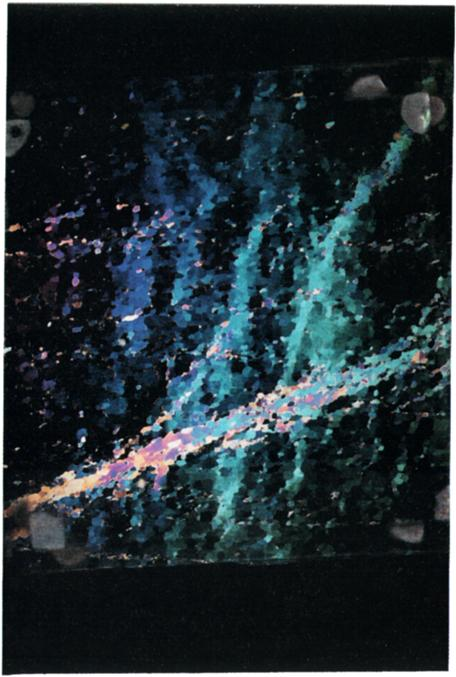
\includegraphics[width=0.5\textheight]{stripes}
     \column{0.3\textwidth}
     \begin{figure}
     \includegraphics[width=\textwidth]{z_fold}
     \caption{\citet{alley97}}
  \end{figure}
     \end{columns}

\end{frame}

\begin{frame}{Ice is very anisotropic}
  \begin{columns}[T]
   \column{0.5\textwidth}
  \begin{itemize}
  \item Ice deforms mostly be shear parallel to the basal plane.
  \item Other slip systems ~100x harder
  \item If the distribution of grain orientations (orientation distribution function) is random, no problem.
    \pause \item But they usually aren't.
    \pause \item Grains rotate away from the axes of extension $\rightarrow$ bulk anisotropic plasticity.
  \item This can cause bulk flow to be highly anisotropic.
  \end{itemize}
  \begin{figure}
     \includegraphics[width=0.5\textwidth]{poly}
     \caption{Rotation of a grain in uniaxial compression}
  \end{figure}
  \column{0.5\textwidth}
  \begin{figure}
     \includegraphics[width=1\textwidth]{ice}
     \caption{Ice crystal structure. (Cappicioti et al.)}
  \end{figure}
  \end{columns}
\end{frame}

\subsection{Different kinds of disturbances}
\begin{frame}{Shear bands and boudinage}
   \begin{columns}[T]
      \column{0.6\textwidth}
   \begin{itemize}
      \small{
      \item Under both horizontal simple shear and uniaxial compression, c-axes go to vertical.
      \item The ice is soft in simple shear because the shear is along the basal plane
      \item A layer that is initially softer will shear faster, and get softer faster
      $\rightarrow$ a shear band.
   }
      \item It's opposite with vertical compression: No shear on horizontal basal planes.
   \end{itemize}
  \column{0.4\textwidth}
   \begin{figure}
      \includegraphics[width=1\textwidth]{drawing}
      \caption{Boudinage under horizontal extension. (a) Undeformed strong layer within weak layers. (b) Necking as the strong layer is pulled apart.}
   \end{figure}
 
\end{columns}
\end{frame}

\begin{frame}{Shear bands and boudinage}
   \begin{figure}
      \includegraphics[width=0.4\textwidth]{shear_band}
      \caption{Shear banding in sand under uniaxial compression. Initial shearing in a layer causes runaway strain.}
   \end{figure}
\end{frame}



\begin{frame}{Layer folding}
   \begin{itemize}
      \item Shear overturns incipient wrinkles, horizontal extension flattens them.
      \item \citet{alley97} showed that anisotropy exacerbates this by making ice soft in shear and hard in uniaxial compression.
      \item Incipient wrinkles could be caused by stripes, or transient flow.
   \end{itemize}
   \begin{figure}
      \includegraphics[height=0.33\textheight]{kinfold}
      \caption{\citet{throstur2002}}
   \end{figure}
\end{frame}

\begin{frame}{Quantifying fabric}
   \begin{columns}[T]
      \column{0.5\textwidth}
      \begin{itemize}\small{
      \item The orientation tensor for a single grain is $c \otimes c$.
      \item The orientation tensor for a collection of grains or a continuous orientation distribution function is $\mathbf{A}^{(2)} = < c \otimes c>$
      \item The strength of a fabric, and its principal orthogonal directions (strongest, middle, weakest) are the eigenvalues and eigenvectors of $\mathbf{A}^{(2)}$.
      }
   \end{itemize}
  \column{0.5\textwidth}
   \begin{figure}
     \includegraphics[width=0.7\textwidth]{eigs}
      \caption{\tiny{C-axes on the unit sphere. The red lines are the eigenvectors scaled by the corresponding eigenvalues}}
   \end{figure}
 \end{columns}
\end{frame}

\begin{frame}{Quantifying fabric}
      \begin{itemize}
      \item Fabric is plotted with Schmidt plots: The c-axes on the hemisphere are flatted down to an equal-area projection.
   \end{itemize}
 
   \begin{figure}
      \includegraphics[height=0.5\textheight]{sm}
      \caption{Schmidt plot of a fabric. The vertical axis comes out of the screen.}
   \end{figure}
\end{frame}

\section{Current work}

\subsection{Ice fabric evolution}

\begin{frame}{Fabric evolution}
   \begin{itemize}
      \item Ice fabric is the properties of a polycrystal (orientations, radii, etc). 
      \item This changes over time in response to stress, temperature, and other factors.
      \item During strain, c-axes rotate away from axes of extension. They also get rotated by any bulk vorticity.
   \end{itemize}
   \begin{figure}
      \includegraphics[width=0.5\textwidth]{crystals}
   \caption{\tiny{Ice sheet thin sections (Center for Ice and Climate, Univ. of Copenhagen. Like colors indicate similar c-axis orientations (L) Shallow ice. (R) Deeper ice.}}
\end{figure}
\end{frame}


\begin{frame}{Normal grain growth}
   \begin{itemize} \small{
      \item Average grain size increases with depth, until polygonization and recrystallization become important.
      \item This is driven by curvature energy: Highly curved interfaces have a lot of free energy $\rightarrow$ small grains shrink
      \item Large grains eat smaller grains. Average grain size increases.
      }
   \end{itemize}



\begin{tikzpicture}[
    tangent/.style={
        decoration={
            markings,% switch on markings
            mark=
                at position #1
                with
                {
                    \coordinate (tangent point-\pgfkeysvalueof{/pgf/decoration/mark info/sequence number}) at (0pt,0pt);
                    \coordinate (tangent unit vector-\pgfkeysvalueof{/pgf/decoration/mark info/sequence number}) at (1,0pt);
                    \coordinate (tangent orthogonal unit vector-\pgfkeysvalueof{/pgf/decoration/mark info/sequence number}) at (0pt,1);
                }
        },
        postaction=decorate
    },
    use tangent/.style={
        shift=(tangent point-#1),
        x=(tangent unit vector-#1),
        y=(tangent orthogonal unit vector-#1)
    },
    use tangent/.default=1
]
\draw [
    tangent=0.6,
    tangent=0.8
] (0,0)
    to [out=50,in=120] (5,2)
    to [out=-60, in=110] (7,1);
%\draw [blue, thick, use tangent] (-3,0) -- (3,0);
\draw [orange, thick,->, use tangent=1] (0,0) -- (0,-1);
\draw [orange, thick,->, use tangent=2] (0,0) -- (0,1);
\end{tikzpicture}
\end{frame}


\begin{frame}{Polygonization}
\begin{columns}[T]
      \column{0.7\textwidth}
   \begin{itemize}
      \item Poorly oriented grains with a large bending moment can split by polygonization. 
      \item This limits grain growth, and makes the fabric more diffuse.
      \item The model does this by splitting grains if the bending moment gets too large. The new orientations are Fisher-distributed about the original c-axis.
   \end{itemize}
   \column{0.3\textwidth}
   \includegraphics[width=1\textwidth]{tilt}
\end{columns}
\end{frame}



\begin{frame}{Dynamic recrystallization} 
   \begin{columns}[T]
      \column{0.6\textwidth}
      \begin{itemize}
         \item Above about $10^{\circ}$C, dynamic recrytallization is important.
         \item Old, highly strained grains have high strain energy, and get eaten by new grains.
         \item The model does this by probabilistically nucleating new grains. They take initial mass from their neighbors.
      \end{itemize}
            \column{0.4\textwidth}
            \begin{figure}
               \includegraphics[width=1\textwidth]{rex}
               \caption{Hardwick \it{et al.} 1961}
            \end{figure}
         \end{columns}


\end{frame}


     
 

\begin{frame}{Fabric evolution model}
\begin{itemize}
     \item \citet{thorsteinsson2002nni} developed a fabric model including nearest-neighbor interactions between grains.
      \item We have developed a new model for evolution of a finite number of grains.
      \item The model includes generalized nearest neighbor interaction, mass conservation, and recrystallization.
   \end{itemize}
\end{frame}

\begin{frame}{Stress homogenization}
   \begin{itemize}
      \item The bulk stress of the polycrystal has to be partitioned between grains.
      \item I use homogeneous stress, the usual assumption for ice: The stress in every grain is the bulk stress.
      \item Each grain gets its viscosity divided by a softness parameter $\zeta$. Hard grains surrounded by soft grains get a big $\zeta$, because they'd get concentrated stress.
      \item The stress on each grain is rotated randomly by a small amount - essentially diffusion.
      \item Thus, each grain gets different strain.
   \end{itemize}
\end{frame}



\begin{frame}{Neighbors and mass balance}
   \begin{itemize}
      \item Each grain has a number of nearest neighbors in an undirected graph.
      \item This does not have a notion of space (like 2D, 3D); just connectivity between grains.
      \item Grains transfer mass between each other - one grain's loss is another's gain.
      \item Mass flux is determined by the total grain boundary velocity between two grains, and the shared area between those two grains..
   \end{itemize}
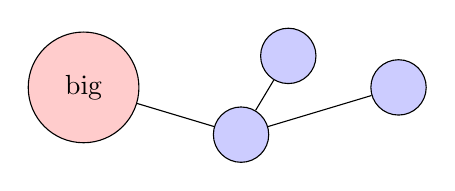
\begin{tikzpicture}[main_node/.style={circle,fill=blue!20,draw,minimum size=2em,inner sep=3pt]},scale=2]

    \node[circle,fill=red!20,draw,minimum size=4em] (1) at (0,0) {big};
    \node[main_node] (2) at (1, -0.3)  {};
    \node[main_node] (3) at (1.3, 0.2) {};
    \node[main_node] (4) at (2,0) {};
    \draw (1) -- (2) -- (3) -- (2) -- (4);
\end{tikzpicture} 
\end{frame}


\begin{frame}{Mass flux}
   \begin{itemize}
      \item Grain-boundary velocity from curvature energy is proportional to the curvature of the interface.
      \item Differences in accumulated strain energy also cause grains to migrate.
      \item Polygonization is handled by splitting a grain into two halves, with half the volume, and changing the orientation of each.
      \item Dynamic recrystallization is done by probabilistically nucleating new grains, taking mass from their neighbors.
      \item If the neighbors are highly strained, the new grain will probably grow.
   \end{itemize}
      \end{frame}

\begin{frame}{Grain rotation and nearest-neighbor interaction}
   Grain rotation is done with by Jeffery's equation \citep{jeffery1922}.
\begin{equation}
   \dot{c_i} &= W_{ij}  c_j + \zeta \left( D^g_{ij} c_j + c_i c_j c_k D^g_{jk} \right), \\
\end{equation}
$W_{ij}$ is the bulk vorticity tensor, $D^g_{ij}$ is the local strain rate tensor of the grain. $\zeta$ is the softness parameter. 
\end{frame}




\begin{frame}{Fabrics}
   The model does a good job at reproducing various fabric types, like girdles and single maximum.

\begin{figure}
   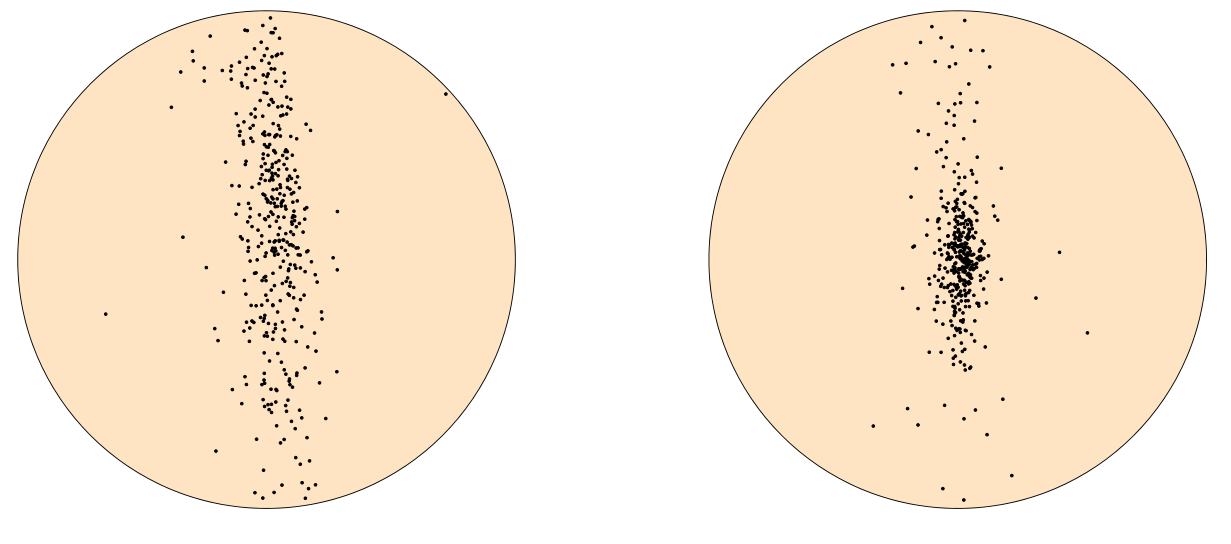
\includegraphics[height=0.5\textheight]{both}
      \caption{\small{Girdle (left) and single maximum fabrics produced from uniaxial compression and simple shear, respectively}}
\end{figure}
\end{frame}

\begin{frame}{Comparison to WAIS ice core}
   \begin{itemize}
         \small{
      \item I forced the model with temperature and velocity from the WAIS divide core.
      \item As an initial condition, I used randomly selected grains from the top thin section at WAIS from Don Voigt.
      \item The model does a pretty good job of fitting the core, capturing the transition from girdle to single maximum, as well as the onset of recrystallization.
      }
   \end{itemize}
\end{frame}
\begin{frame}
   \begin{figure}
   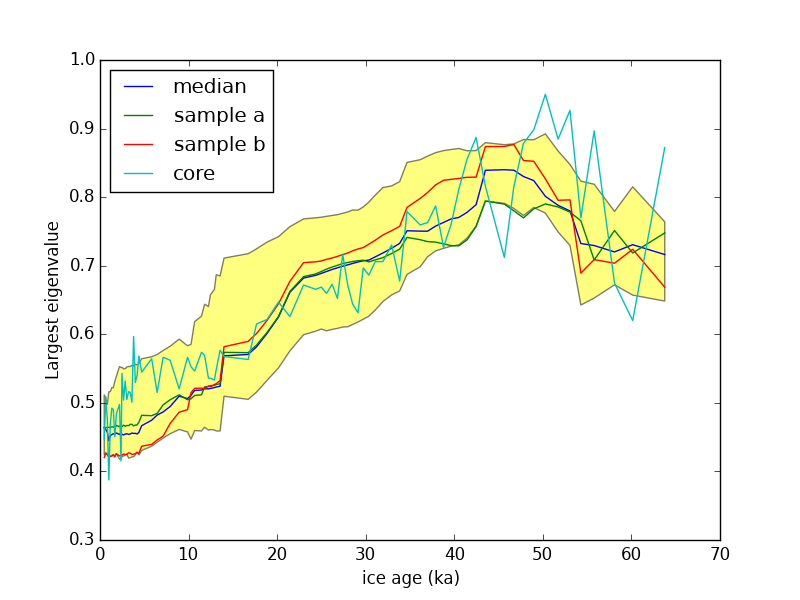
\includegraphics[width=1\textwidth]{good_fit}
   \caption{Largest eigenvalues of modeled and observed fabric thin sections through the WAIS core. The shaded area is the 95\% interval of all model runs. Two individual runs are included.}
\end{figure}
\end{frame}

\subsection{Coupled anisotropic ice flow/fabric evolution}
\begin{frame}{Flow and fabric}
      \begin{itemize} \small{
   \item Ice fabric development is driven by flow, so this is a coupled system.
   \item Stokes flow with fiber inclusions (similar to ice) is unstable to pertubrations in the ODF \citep{montgomery-smith2011}.
   \item \citet{gillet2006} found large-scale stratigraphic disruptions in a numerical model.
   \item Can an initial random perturbation become a strong perturbation?
   }
\end{itemize} 
\begin{figure*}
   \includegraphics[height=0.5\textheight]{grip_gillet}
   \caption{\tiny{\\ A33 component of second-order orientation tensor. (a) initial; (b) steady state \citet{gillet2006}}}

\end{figure*}
\end{frame}


\begin{frame}{The flow model}
   \begin{itemize}
      \item The General Orthotropic Linear Flow (GOLF) law \citep{gillet2005} is a constitutive relation depending on six viscosity parameters.
      \item It assumes the ODF is orthotropic (three axes of symmetry).
      \item Under some assumptions, I found an expression for the fabric parameters in terms of the fabric eigenvalues.
   \end{itemize}
   \begin{equation}
   S_{ij} = \eta_0 \left[ \eta_r M_{rkl} D_{kl} \left( M_{rij}^D \right)  + \eta_{r+3} \left( D_{ik} M_{rkj} + D_{kj} M_{rik} \right)^D \right],
   \end{equation}
\end{frame}

\begin{frame}{Fabric evolution}
   %closure approx
   \begin{itemize}
      \item I use a tensor-closure approximation for Jefferys equation. This very common in fiber injection molding modeling. 
      \item $\mathbf{A}^{(2)}= < c \otimes c>$ is the second order orientation tensor. 
   \end{itemize} \\
   \begin{equation}
      \frac{\partial A_{ij}}{\partial t} = -\frac{\partial}{\partial x_k} A_{ij} u_k + W_{ik} A_{kj} - A_{ik} W_{kj} - (D_{ik}W_{kj} + D_{kj}W_{ik}) + 2 \mathbb{A}_{ijkl} C_{kl}
   \end{equation}

\end{frame}

\begin{frame}{Setup and perturbations}
   \begin{itemize} 
      \item I assume an infinite 3D space with an unperturbed velocity gradient $U_{ij}$.
      \item Fabric is spatially homogeneous.
      \item Then, we put in in a small perturbation of $A^{(2)}_{ij}$ with a wavenumber $\kappa_i$.
   \end{itemize}
   \begin{aligned}
   A_{ij} &\rightarrow \bar{A}_{ij} +  \epsilon \hat{A}_{ij} e^{i \kappa_k x_k} \\
      u_j &\rightarrow \bar{U}_{ij}x_j +  \epsilon \hat{u}_j e^{i \kappa_k x_k} \\
      p &\rightarrow \bar{p} + \epsilon \hat{p} e^{i \kappa_k x_k} \\
      S_{ij} &\rightarrow \bar{S}_{ij} +  \epsilon \hat{S}_{ij} e^{i\kappa_k x_k}
   \end{aligned}
\end{frame}

\begin{frame}{Stability}
   \begin{itemize}
      \item Using the previous replacements, the exponential terms go away. It leaves an ODE for $A^{(2)}_{ij}$.
      \item It is a long ODE, but it is nice and linear nonetheless.
      \item This can be used to look at stability of fabric perturbations under many different scenarios.
   \end{itemize}
\begin{equation}
\begin{align*}
   \frac{\partial \hat{A}_{ij}}{\partial t} &= -\kappa_k \hat{A}_{ij} \bar{u_k} + \kappa_k \bar{A}_{ij} \hat{u}_k  + \bar{W}_{ik} \hat{A}_{kj} + \hat{W}_{ik} \bar{A}_{kj}  - \bar{A}_{ik} \hat{W}_{kj} 
  \\ 
   &- \hat{A}_{ik} \bar{W}_{kj} - \hat{D}_{ik}\bar{W}_{kj} - \bar{D}_{ik}\hat{W}_{kj} 
   \\ 
   & - \hat{D}_{kj}\bar{W}_{ik} - \bar{D}_{kj} \hat{W}_{ik} + 2 (\bar{\mathbb{A}}_{ijkl} \hat{D}_{kl} + \hat{\mathbb{A}}_{ijkl} \bar{D}_{kl})
\end{align*}
\end{equation}.
\end{frame}

\section{Future work}

\begin{frame}{Other analytical ideas}
   \begin{itemize}
      \item Stripe growth.
      \item Is boudinage inhibited or helped by anisotropy?
      
   \end{itemize}
\end{frame}


\begin{frame}{Is GOLF sufficient to explain anisotropic flow?}
   \begin{itemize}
      \item Fluids made up of linearly viscous transversely isotropic components do not depend on higher than $4^{th}$ order orientation tensors.
      \item GOLF assumes orthotropy, which does not hold in general for fourth order tensors.
      \item Also, ice is not linear, and nearest-neighber interactions seem to be important for ice.
      \item Does this mean that we need a more general flow model to address these shortcomings? \\
         \pause I don't think so, but maybe.
   \end{itemize}
\end{frame}
\begin{frame}{Is GOLF sufficient to explain anisotropic flow?}
   \begin{itemize}
      \item Nearest neighbor interaction makes a big difference with fabric evolution. Some grains get more than 10x softness.
      \item This only makes for differences of $~1\%$ in bulk viscosity. But is is possible to construct fabrics where it the difference is bigger.
      \item Strain softening might be a similar situation.
      \item I propose investigating this question numerically for different fabrics. This will determine whether it is necessary to expand on GOLF.
      \item Prediction of fabric orientation would be improved by a higher-order evolution equation, either up to the sixth-order orientation tensor or using spherical harmonics.
   \end{itemize}
\end{frame}
\begin{frame}{Numerical flow modeling}
   \begin{itemize}
      \item To expand things beyond first order, I propose investigating mesoscale anisotropic flow with a 3d model in a box geometry.
      \item We can user Elmer/Ice FEM with the GOLF flow law.
      \item If we roll our own, we would use a simple finite volume scheme. Numerically, it is similar to to standard Stokes flow.
   \end{itemize}
\end{frame}

\begin{frame}{Outlook}
   \begin{itemize}
      \item We will submit the paper on the fabric model shortly.
      \item The perturbatative coupled model will form another paper.
      \item The work on constitutive relations and numerical flow modeling will make for a total of three or four.
      \item I am funded on NSF Grant 0636996 through June 2016.  
      \item I anticipate finishing in 2016.
   \end{itemize}
\end{frame}


% All of the following is optional and typically not needed. 
\appendix
\section<presentation>*{\appendixname}
\subsection<presentation>*{For Further Reading}

\begin{frame}[allowframebreaks]
  \frametitle<presentation>{References}
    
  %\beamertemplatebookbibitems
  % Start with overview books.
  \bibliographystyle{igs}
  \bibliography{anis}
\end{frame}

\end{document}


